\documentclass[a4paper, 11pt, fleqn, normalem]{report}

\usepackage{../../../LaTeX-Templates/Notes}

\titlecontents{chapter}% <section-type>
    [0pt]% <left>
    {}% <above-code>
    {Lecture \thecontentslabel\quad}% <numbered-entry-format>
    {}% <numberless-entry-format>
    {\dotfill\contentspage}% <filler-page-format>
\titleformat{\chapter}{\fontsize{13}{15}\bfseries\normalfont}{\textbf{Lecture \thechapter}}{1em}{}
\setcounter{tocdepth}{1}
\setcounter{secnumdepth}{1}

\title{Foundations of Physics Year 1 \\ Electromagnetism \vspace{-20pt}}
\author{Ian Terry \& Marek Szablewski}
\date{\vspace{-15pt}Epiphany Term 2017}
\rhead{\hyperlink{page.1}{Go to TOC}}

\begin{document}

\maketitle
\thispagestyle{fancy}

\tableofcontents

\part{Electrostatics}
\chapter{}
\section{Electrostatics}
A class of phenomena which is recognised by: \\
(i) The presence of electrical charges, either stationary or moving; \\
(ii) Interactions between these charges
\begin{itemize}
    \item SI unit of charge is the Coulomb, C
    \item Symbol for charge is q/Q
\end{itemize}
Two types of charge are found in nature -- positive and negative \\
Like charges repel one another; opposite charges attract

Law of conservation of charge:
\begin{equation*}
    \sum q = k
\end{equation*}
Materials can be:
\begin{itemize}
    \item Conductors -- charge is free to move
    \item Insulators -- charge is localised
\end{itemize}

\section{Coulomb's Law}
Describes the force between electric charges \\
Consider charges $q_{1}$ and $q_{2}$: \\
Positions are defined by the position vectors $\vec{r}_{1}$ and $\vec{r}_{2}$ \\
Vector distance separating charges is $\vec{r}_{12} = \vec{r}_{2} - \vec{r}_{1}$ \\
Coulomb observed that force acts along the line joining charges so the force on $q_{2}$ due to $q_{1}$, $\vec{F}_{1on2}$, is along $\vec{r}_{12}$ \\
The unit vector directed from $q_{1}$ to $q_{2}$ is:
\begin{gather*}
    \hat{r}_{12} = \frac{\vec{r}_{12}}{|\vec{r}_{12}|},~~~|\vec{r}_{12}| = r_{12} \\
    \vec{F}_{1on2} = k\frac{q_{1}q_{2}}{r_{12}^{2}},~~~\vec{F}_{2on1} = -\vec{F}_{1on2} \\
    k = 8.988\times10^9\text{ N m}^{2}\text{ C}^{-2} \\
    k = \frac{1}{4\pi\epsilon_{0}} \\
    \epsilon_{0} := \text{Permittivity of free space} \\
    \epsilon_{0} = 8.854\times10^{-12}\text{ C}^{2}\text{ m}^{-2}\text{ N}^{-1}
\end{gather*}
This is true for charges in a vacuum, but air is not that different

\chapter{}
\section{Superposition of Electrostatic Forces}
Consider a three charge system:
\begin{figure}[H]
    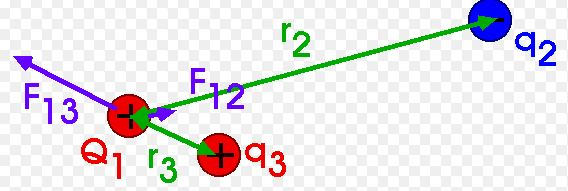
\includegraphics{3Force.jpg}
\end{figure}
Net force on $Q_{1}$:
\begin{equation*}
    \vec{F}_{T} = \vec{F}_{13} + \vec{F}_{12}
\end{equation*}
Using Coulomb's Law:
\begin{equation*}
    \vec{F}_{T} = k\Big[\frac{q_{1}q_{3}}{r_{13}^{2}}\hat{r}_{13} + \frac{q_{1}q_{2}}{r_{12}^{2}}\hat{r}_{12}\Big]
\end{equation*}
Generalising to n charges:
\begin{equation*}
    \vec{F}_{T} = \sum_{i = 1}^{n} \vec{F}_{i\,on\,0},~~n \in \mathbb{N}
\end{equation*}

\textbf{Example: }
\begin{table}[H]
    \begin{tabular}{|c|c|c|}
    \hline
    \rowcolor{lightgray} & Charge & Position Vector \\
    \hline
    $q_{0}$ & $-0.5\times10^{-9}$\,C & $\vec{r}_{0} = 5\,\text{cm}\hat{j}$\\
    \hline
    $q_{1}$ & $1\times10^{-9}$\,C & $\vec{r}_{1} = -0.1\,\text{cm}\hat{i}$\\
    \hline
    $q_{2}$ & $-1\times10^{-9}$\,C & $\vec{r}_{2} = 0.1\,\text{cm}\hat{i}$\\
    \hline
    \end{tabular}
\end{table}
Coulomb:
\begin{gather*}
    \vec{F}_{0} = k\Bigg[\frac{q_{1}q_{0}}{r_{10}^{2}}\hat{r}_{10} + \frac{q_{2}q_{0}}{r_{20}^{2}}\hat{r}_{20}\Bigg] \\
    \hat{r}_{10} = 0.1\hat{i} + 5\hat{j} ~~~~ \hat{r}_{20} = -0.1\hat{i} + 5\hat{j} \\
    |r_{10}| = |r_{20}| \approx 5\,\text{cm} \\
    \hat{r}_{10} = 0.02\hat{i} + \hat{j} ~~~~ \hat{r}_{20} = -0.02\hat{i} + \hat{j}
\end{gather*}
$q_{1}$ and $q_{2}$ act as an electric dipole
\begin{gather*}
    \vec{F}_{0} = k\frac{q_{1}q_{0}}{r_{10}^{2}}\Big[\hat{r}_{10} - \hat{r}_{20}\Big] \\
    ~~~~ = 9\times10^{9} \cdot \frac{1\times10^{-9}\times0.5\times10^{-9}}{25}\Big[4\times10^{-2}\hat{i}\Big] \\
    ~~~~ = -1.8\times10^{-6}\,N\,\hat{i}
\end{gather*}

\section{Electric Field}
A charge modigies properties of space around it, the modification being described by an electric field, $\vec{E}$ \\
Electric field describes the force per unit charge at a point in space due to a fixed charge
\begin{equation*}
    \vec{E} = \frac{\vec{F}}{q_{0}}
\end{equation*}
Units are N C$^{-1}$ \\
It is a vector field \\
Charges placed in an electric field experience $\vec{F} = q\vec{E}$ \\
$\vec{E}$ reacts instantaneously to the change in charge producing it \\
Superposition of electric field at a point of space means field addition is possible

\chapter{}








































































































































































































































































































































































































\end{document}
